\subsection{Feature Extraction}
In previous motif mining research \cite{shao2013temporal}, 
a smoothing window is used to extract the steady states of power levels.
However for continuously variable loads, such as heating units, 
it takes more than 40 seconds to preheat then stays at 
a steady state.  
For variable water usage device, for instance toilet, 
the water flow rate only stays in a steady state for several seconds, 
then gradually drops to zero. 
Motif mining has advantage in dealing with discrete events, but 
lacks of capability in finding the variable load or water usage devices. 
In this chapter, we extract more features, including the previous used 
power level, and newly added on/off startup duration and shape. 
In order to obtain these features, 
we preprocess a period's on/off events from the ground truth data with the aggregated data 
to compute the power levels, on/off startup duration and shape for 
each water use end or electric device.
%This process is a key step for episode mining. 
 
Due to deviation of sensors, the timestamp of the aggregated data and
sensor data of each device may not synchronize so well. 
Figure \ref{fig_humidifierSyn} shows three situations of
the aggregated data and actual start time of a humidifier. 
In Figure \ref{fig_humidifierSyn} (a), 
the actual on event of the humidifier occurs just in the middle of on
event of aggregated data, i.e. good synchronization.
However, Figure \ref{fig_humidifierSyn} (b) and (c) indicate that the
actual on event lags behind or goes ahead of aggregated data. 
This difference of time stamp synchronization between 
the aggregated data and actual events 
hinders us from extracting the power levels of each device accurately.
\begin{figure}[!t]
\centering
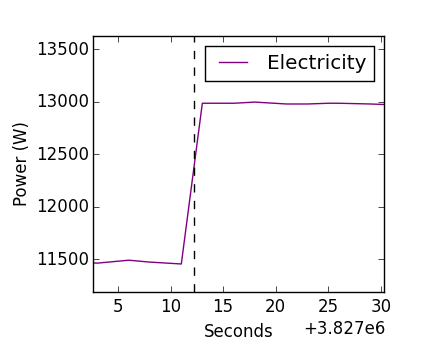
\includegraphics[width=2.5in]{multidisaggfigs/humidifierSyn1.png}
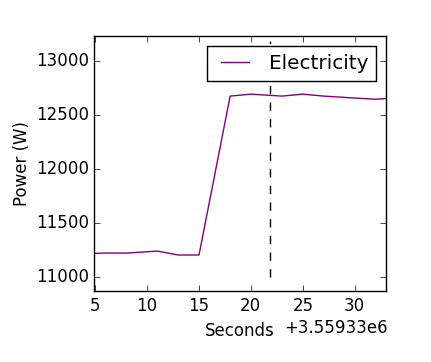
\includegraphics[width=2.5in]{multidisaggfigs/humidifierSyn2.png}
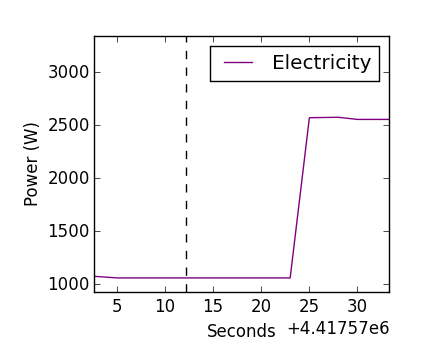
\includegraphics[width=2.5in]{multidisaggfigs/humidifierSyn3.png}
\caption{Difference synchronization time of the same device humidifier in dataset study 10. Where the vertical dash line represents the start time of humidifier.}
\label{fig_humidifierSyn}
\end{figure}

Therefore, we introduce window size in the feature extraction algorithm as described 
in Algorithm \ref{alg_extractFeatures}, which describes how the features of 
the power or water are extracted.
The input includes a snippet of aggregated data over a short period of time $(t1,..., t_n)$, the ground truth on/off events $(e_1, ...., e_m)$ of each device $m$ during the same period, 
the window size, which helps evaluate whether a specific event is 
caused by the operation a single device or not. 
The output include the usage levels and its standard deviation, 
on/off duration of each device. 

Initially from the aggregated data $y=(t_1, y_1,..., t_n, y_n)$, we build 
a linked list $L1<t,y>$, where $t$ is the time stamp, 
$v$ is the power consumption or water flow rate. 
Then from the on/off ground truth events $(t_1, e_1, ..., t_m, e_m)$, 
we create another linked list $L2<t,set(e)>$, where 
$t$ is the time stamp, and $set(e)$ is a set of events which occurs at time $t$. 
From line $5$ to line $10$, 
all the events in the events list $L2$ are iterated to check 
whether the gap duration between any two events are less than the threshold $\Delta t$. 
If the gap is smaller than $\Delta t$, that means these two events 
infer with each other, then both of these two events are deleted from $L2$. 
Then we delete those nodes in $L2$, where there are more than one events in that node. 
For each time event $t_j$ in $L2$, we set a time range $(t_j-\Delta t, t_j+\Delta t)$. 
Then we search all the values in $L1.y$ where $L1.t \in (t_j-\Delta t, t_j+\Delta t)$
and obtain a series of values in in $(y_j, ....y_{j+2\Delta t})$. 
If there is only one value in this list, that means there is no usage level change, 
no corresponding event in the aggregated data matching the ground truth event in $L2$. 
If this event is an on event and $y_{j+2\Delta t} - y_j > 0$, or 
if the event is an off event and $y_{j+2\Delta t} - y_j < 0$, keep this event as a ground truth event for a corresponding device $m$. 
$set(P_{m}).add(y_{j+2\Delta t} - y_j)$.
At last, we apply Gaussian mixture model to the usage level diffs set $set(P_m)$ of each device $m$ 
to compute the mean values as usages levels $P_m$, 
standard deviation as $P_m^{std}$. 
The on/off event duration is computed as the minimal gap $D_m= j''- j' $, where in ${y_j , ...y_{j+j'},..., y_{j+j''} y_{j+2\Delta t}}$, 
$y_j, ..., j_{j+j'}$ are the same values and $y_{j+j''}, ..., j_{j+2\Delta t}$ are the same.

\begin{algorithm}
\caption{Feature Extraction}
\begin{algorithmic}[1] 
\label{alg_extractFeatures}
\REQUIRE a snippet of aggregated data $y= (t_1, y_1,...,t_n, y_n)$, ground truth events $(t_1, e_1, ..., t_k, e_k)$, 
window size $\Delta t$ 
%\ENSURE $y = x^n$
\STATE create $L1<t, v>$
\STATE create $L2<t,set(e)>$
\STATE $cur=L2.head, post= cur.next$
\WHILE{$post.next!=null$ \& $post.next.next!=null$}
\IF {$post.t - cur.t < \Delta t$}
\STATE $newCur=post.next$
\STATE $L2.remove(cur)$, $L2.remove(post)$
\STATE $cur= newCur$, $post=cur.next$
\ENDIF
\ENDWHILE
\WHILE{$len(node.set(e))!=1$}
\STATE $L2.remove(node)$
\ENDWHILE
\STATE $cur=L2.head$
\WHILE{cur!=null}
\STATE search $L1.t \in (cur.t-\Delta t, cur.t+\Delta t)$. 
\IF {$y_{j+2\Delta t} - y_j > 0$ and $cur.e$ is on event}
\STATE $P_{m}.add(y_{j+2\Delta t} - y_j)$
\ENDIF
\IF {$y_{j+2\Delta t} - y_j < 0$ and $cur.e$ is on event}
\STATE $Set(P_{m}).add(y_{j+2\Delta t} - y_j)$
\ENDIF
\ENDWHILE
\STATE GMM to $set(P_m)$
\RETURN $P_m$, $P_m^{std}$ and $D_m$
\end{algorithmic}
\end{algorithm}

In order to extract the usage levels of all devices of power or water, 
we increase the window size from 5 seconds to one minutes 
to compare the usage level results. 
Usually, when the window size is small, 
the usage levels of devices which starts in a very short period of time 
can be clustered clearly. 
When the window size is large as $60$ seconds, 
the usage levels of continuously variable loads can be 
found and clustered explicitly. 

For continuously variable loads, such as indoor heating, 
we extract the startup shape $y_{j+j'}, ..., y+{j+j''}$ as a feature. 
For some water end use such as toilet, which operates for a very short period of time 
and its usage levels changes for several times, 
we obtain the whole cycle as a feature other than only the startup or shutdown shape.
